\documentclass[12pt]{ucthesis}

\usepackage{etex}
\usepackage[morefloats=125]{morefloats}
\usepackage[hyphens]{url}
\usepackage{subfig}
\usepackage{graphicx}
\usepackage{amssymb}
\usepackage{amsmath}
\usepackage[letterpaper]{geometry}
\usepackage[overload]{textcase}
\usepackage{color}
\usepackage[nonumberlist,toc]{glossaries}
\usepackage{wrapfig}
\usepackage{morefloats}
\usepackage{float}
\usepackage{listings}
\usepackage{makecell}
\usepackage{appendix}
\usepackage[]{algorithm2e}
\usepackage{titlesec}
\usepackage[breaklinks=true,hidelinks,pdfusetitle]{hyperref}
\usepackage{cleveref}
\usepackage{ifthen}

\usepackage{siunitx}
\usepackage{pdfpages}
\usepackage{pdflscape}
\usepackage{xcolor}
%\usepackage{setspace}

% Table related packages
%\usepackage{longtable}
%\usepackage{tabularx}
\usepackage{ltxtable}
\captionsetup[longtable]{labelfont=bf,textfont=bf}
\usepackage{booktabs}
\usepackage{ragged2e}  % for '\RaggedRight' macro (allows hyphenation)
\newcolumntype{Y}{>{\RaggedRight\arraybackslash}X} 

\makeindex
\makeglossaries

% Shrink the size of headers
\titleformat{\chapter}[display]
        {\normalfont\normalsize\centering}
        {\ifthenelse{\equal{\thechapter}{A}}{APPENDICES\\[4.3ex]}{}\chaptertitlename\ \thechapter}
        {0pt}{\normalsize\uppercase}
\titlespacing*{\chapter}{0pt}{-20pt}{4.3ex plus .2ex}


\titleformat*{\section}{\normalsize\bfseries}
\titleformat*{\subsection}{\small\bfseries}
\titleformat*{\subsubsection}{\small\bfseries}
\titleformat*{\paragraph}{\small\bfseries}
\titleformat*{\subparagraph}{\small\bfseries}

% Python formatting ~~~~~~~~~~~~~~~~~~~~~~~~~~~~~~~~~~~~~~~~~~~~~~~
% Default fixed font does not support bold face
\DeclareFixedFont{\ttb}{T1}{txtt}{bx}{n}{12} % for bold
\DeclareFixedFont{\ttm}{T1}{txtt}{m}{n}{12}  % for normal

% Custom colors
\usepackage{color}
\definecolor{deepblue}{rgb}{0,0,0.8}
\definecolor{deepred}{rgb}{0.8,0,0}
\definecolor{deepgreen}{rgb}{0,0.8,0}
\definecolor{gray}{rgb}{0.4,0.4,0.4}

\usepackage{linegoal}

% Fixes inline wrapping issue, see https://tex.stackexchange.com/questions/56361/avoid-linebreak-in-lstinline-if-possible
\newsavebox{\mylisting}
\makeatletter
\newcommand{\lstInline}[2][,]{%
  \begingroup%
  \lstset{#1}% Set any keys locally
  \begin{lrbox}{\mylisting}\lstinline!#2!\end{lrbox}% Store listing in \mylisting
  \setlength{\@tempdima}{\linegoal}% Space left on line.
  \ifdim\wd\mylisting>\@tempdima\hfill\\\fi% Insert line break
  \lstinline!#2!% Reset listing
  \endgroup%
}
\makeatother

% C style
\newcommand\cstyle{\lstset{
	language=C,
	basicstyle=\ssp\ttfamily\scriptsize,
	frame=tb, % draw a frame at the top and bottom of the code block
 	tabsize=3, % tab space width
	showstringspaces=false, % don't mark spaces in strings
	numbers=left, % display line numbers on the left
	commentstyle=\color{deepgreen}, % comment color
	keywordstyle=\color{deepblue}, % keyword color
	stringstyle=\color{deepred}, % string color
	breaklines=true
}}

% C style for inline
\newcommand\cstyleinline{\lstset{
	language=C,
	basicstyle=\ssp\ttfamily,
 	tabsize=3, % tab space width
	showstringspaces=false, % don't mark spaces in strings
	commentstyle=\color{deepgreen}, % comment color
	keywordstyle=\color{deepblue}, % keyword color
	stringstyle=\color{deepred}, % string color
	breaklines=true
}}

% Command for inline C
\newcommand\cinline[1]{{\cstyleinline\lstInline{#1}}}

% C environment
\lstnewenvironment{clisting}[1][]
{
	\cstyle
	\lstset{#1}
}
{}

% Python style for highlighting
\newcommand\pythonstyle{\lstset{
		language=Python,
		basicstyle=\ssp\ttfamily\scriptsize,
		otherkeywords={self},             % Add keywords here
		keywordstyle=\color{deepblue},
		emph={MyClass,__init__},          % Custom highlighting
		emphstyle=\color{deepred},    % Custom highlighting style
		stringstyle=\color{deepgreen},
		numbers=left,
		commentstyle=\color{gray}, % comment color
		frame=tb,                         % Any extra options here
		showstringspaces=false,            % 
		tabsize=3, % tab space width
		breaklines=true
}}

% Python style for inline
\newcommand\pythonstyleinline{\lstset{
		language=Python,
		basicstyle=\ssp\ttfamily,
		otherkeywords={self},             % Add keywords here
		keywordstyle=\color{deepblue},
		emph={MyClass,__init__},          % Custom highlighting
		emphstyle=\color{deepred},    % Custom highlighting style
		stringstyle=\color{deepgreen},
		commentstyle=\color{gray}, % comment color
		showstringspaces=false,            % 
		tabsize=3, % tab space width
		breaklines=true
}}

% Python environment
\lstnewenvironment{python}[1][]
{
	\pythonstyle
	\lstset{#1}
}
{}

% Python for external files
\newcommand\pythonexternal[2][]{{
		\pythonstyle
		\lstinputlisting[#1]{#2}}}

% Python for inline
\newcommand\pythoninline[1]{{\pythonstyleinline\lstinline!#1!}}



\bibliographystyle{abbrv}

\setlength{\parindent}{0.25in} \setlength{\parskip}{6pt}
\geometry{verbose,nohead,tmargin=1in,bmargin=1in,lmargin=1.5in,rmargin=1in}
\setcounter{tocdepth}{2}

% Different font in captions (single-spaced, bold) ------------
\newcommand{\captionfonts}{\small\bf\ssp}

\newcommand{\mycaption}[2]{\caption[#1 --- #2]{#1 --- #2}}

\makeatletter  % Allow the use of @ in command names
\long\def\@makecaption#1#2{%
  \vskip\abovecaptionskip
  \sbox\@tempboxa{{\captionfonts #1: #2}}%
  \ifdim \wd\@tempboxa >\hsize
    {\captionfonts #1: #2\par}
  \else
    \hbox to\hsize{\hfil\box\@tempboxa\hfil}%
  \fi
  \vskip\belowcaptionskip}
\makeatother   % Cancel the effect of \makeatletter
% ---------------------------------------

% Define Appendix refs
\crefname{app}{appendix}{appendices}
\Crefname{app}{Appendix}{Appendices}

% Rename Table of Listings
\renewcommand{\lstlistlistingname}{LIST OF LISTINGS}
    
\begin{document}

% Declarations for Front Matter
\title{Artificial Neural Network-Based Robotics}
\author{Justin Ng}
\degreemonth{June} \degreeyear{2018} \degree{Master of Science}
\defensemonth{June} \defenseyear{2018}
\numberofmembers{2}
   \chair{Andrew Danowitz, Ph.D. \linebreak Assistant Professor of Electrical Engineering}
   \othermemberA{Xiao-Hua Yu, Ph.D. \linebreak Professor of Electrical Engineering}
   \othermemberB{Fred W. DePiero, Ph.D. \linebreak Professor of Electrical Engineering}
\field{Electrical Engineering} \campus{San Luis Obispo}
\copyrightyears{seven}


\maketitle

\begin{frontmatter}

% Custom made for Cal Poly (by Mark Barry, modified by Andrew Tsui).
\copyrightpage

% Custom made for Cal Poly (by Andrew Tsui).
\committeemembershippage

\begin{abstract}
Artificial neural networks (ANNs) are highly-capable alternatives to traditional problem solving schemes due to their ability to solve non-linear systems with a non-algorithmic approach. The applications of ANNs range from process control to pattern recognition and, with increasing importance, robotics. This paper demonstrates continuous control of a robot using an actor-critic algorithm based on deep deterministic policy gradients (DDPG) originally conceived by Google DeepMind. The robot performs tasks such as locomotion within an enclosed area and object transportation. The paper also details the robot design process and explores the challenges of implementation in a real-time system.
\end{abstract}

\begin{acknowledgements}
\noindent
Thanks:
\begin{itemize}
    \item To Andrew Danowitz for his guidance, support, and time throughout the project. Many thanks!
    \item To my best friend in the world and unwavering fountain of support, Earth Wimolnit. You kept me alive and sane, and I couldn't have done it without you! Thank you and I love you!
\end{itemize}

\end{acknowledgements}

\tableofcontents

\listoftables

\listoffigures
\newpage
\addcontentsline{toc}{chapter}{{LIST OF LISTINGS}}
\lstlistoflistings

% Add CHAPTER into table of contents.
\addtocontents{toc}{%
   \noindent CHAPTER
}

\end{frontmatter}

\pagestyle{plain}

\renewcommand{\baselinestretch}{1.66}

%\chapter{Introduction}

\textbf{Note}: All project files can be found at \url{https://www.github.com/okayjustin/roborodentia2017} \

\section{Definitions and Assumptions}
The robot is designed to only travel within a rectangular closed area of eight feet in the x direction and five feet in the y direction. The coordinate system is chosen as Cartesian with the origin placed at the bottom-left corner of the field. The position of the robot is always in the xy-plane since it cannot move vertically (z = 0). Therefore, $x$ refers to the robot position along the x-axis and ranges from 0 to 8 feet, and $y$ refers to position along the y-axis and ranges from 0 to 5 feet. Additionally, the robot can only rotate around the z-axis so $\theta$ refers to the angle of the robot in the xy-plane. Maintaining standard Cartesian coordinates, $\theta=\ang{0}$ is along the positive x direction while $\theta=\ang{90}$ is along the positive y direction.

\section{Cal Poly Roborodentia}
The robot is designed to compete in the 2018 Cal Poly Roborodentia, the university's annual intramural robotics competition, and thus conforms to its particular specifications and requirements. Briefly, autonomous robots collect and fire Nerf Rival Balls into nets to win points. A drawing of the field is shown below in Figure  \ref{fig:roborodentia_field}. 

\begin{figure}[H]   % [h] means here
	\centering
	\includegraphics[width=7in]{figures/roborodentia_field.png}
	\caption{Roborodentia Field}
	\label{fig:roborodentia_field}
\end{figure}




%\chapter{Mechanical Design}
The robot meets the Roborodentia design requirements shown in Table \ref{tab:roborodentia_reqs}. It consists of four subassemblies: the base platform, shooting mechanism, ball hopper, and control unit. Each section was modeled in SolidWorks, an industry-standard solid modeling CAD program \cite{solidworks}. The parts were fabricated using a laser cutter or 3D printer and assembled with metric hardware. Figure \ref{fig:robot_photo} displays a photograph of the robot while Figures \ref{fig:render_isometric} through \ref{fig:render_right} show standard view renders of the SolidWorks model. Note that the robot uses mecanum wheels (a type of omni-directional wheel) \cite{ilon_1975} which are modeled as plain wheels for simplicity. Figure \ref{fig:render_top} also indicates the front, left, back/rear, and right sides of the robot. The robot contains 53 different mechanical components (including fasteners and off-the-shelf parts), of which 24 are custom designed, and 394 parts in total. The bill of materials can be found in Appendix \ref{appendix:mech_bom}.

\begin{table}[h]
	\caption{Roborodentia 2018 Mechanical Requirements}  \label{tab:roborodentia_reqs}
	\begin{tabularx}{\textwidth}{@{} c Y @{}}
		\toprule
		& Requirement \\ 
		\midrule
		1. & Maximum footprint of 12" x 14" or smaller at start of match but may expand up to 14" x 17" during match. \\
		2. & Maximum height of 14" at start of match but no restriction during match. \\ 
		3. & Robot may not disassemble into multiple parts. \\ 
		4. & Robot may not be airborne. \\ 
		5. & Shooting mechanisms may not accelerate balls past 50 feet per second. \\ 
		\bottomrule
	\end{tabularx} 
\end{table}

\begin{figure}[H]   % [h] means here
	\centering 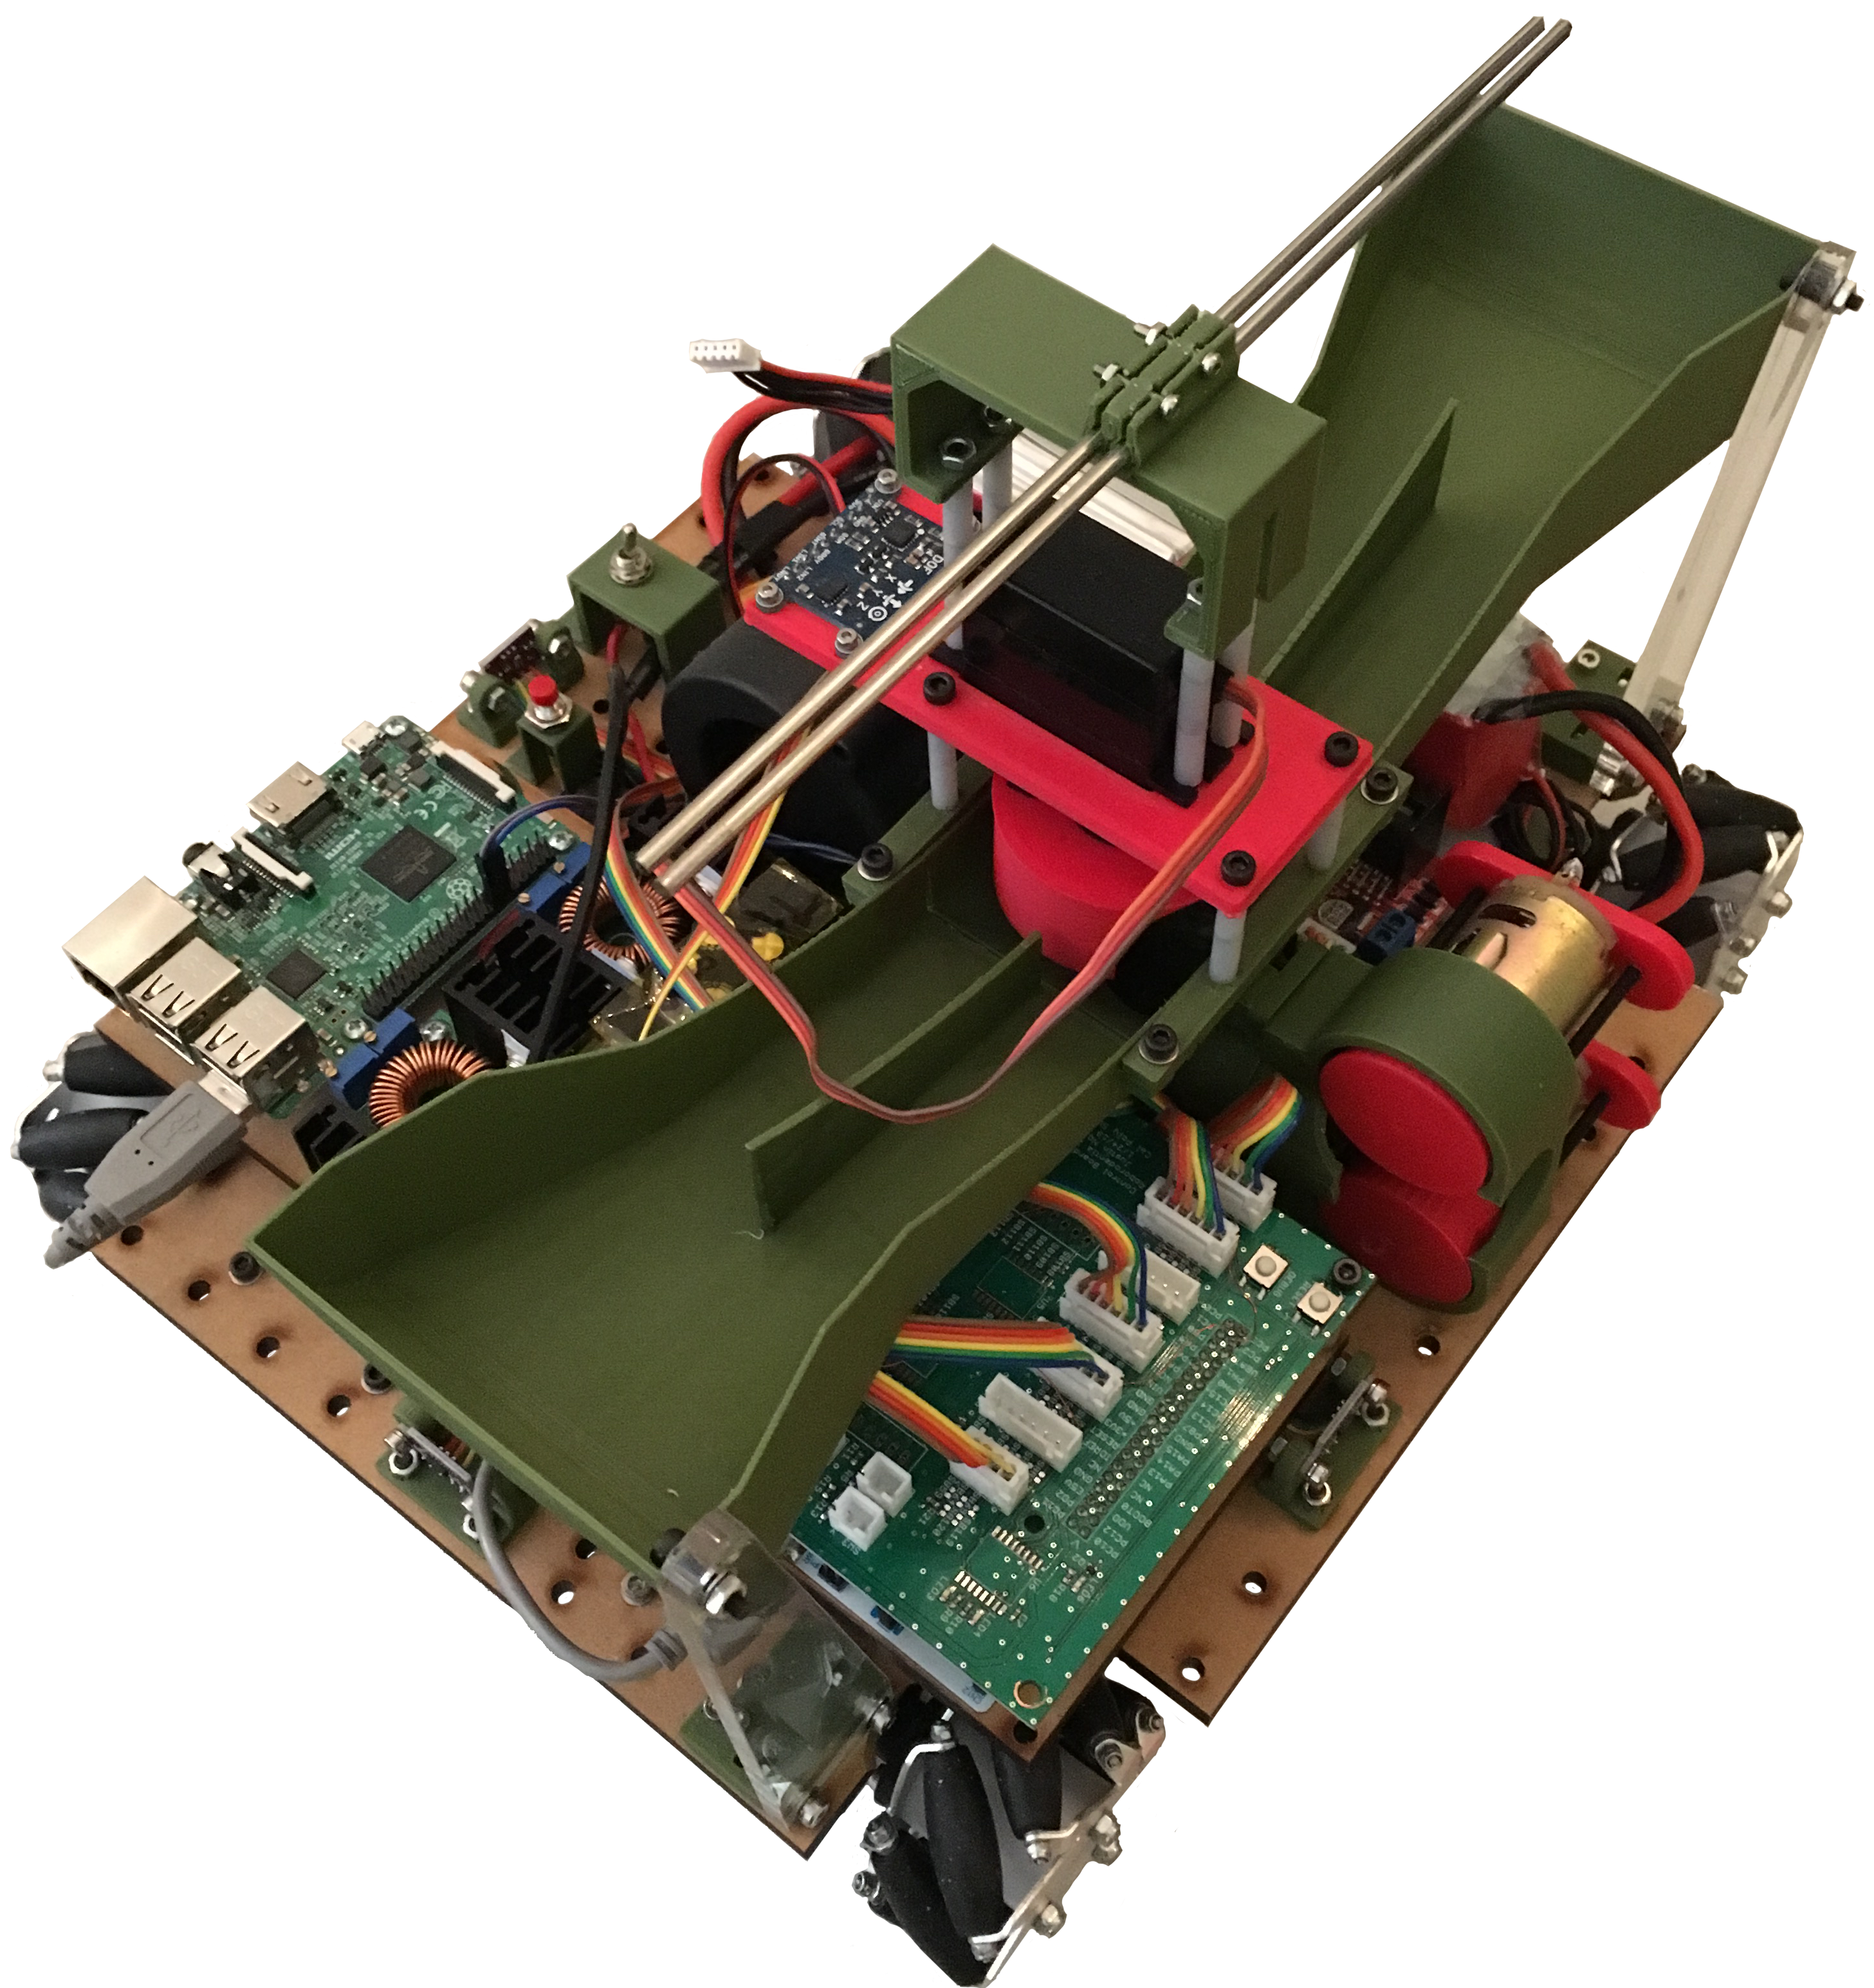
\includegraphics[width=6in, height=7in, keepaspectratio]{figures/robot_photo.png}
	\caption{Photograph of Robot}	\label{fig:robot_photo}
\end{figure}
\begin{figure}[H]   % [h] means here
	\centering \includegraphics[width=6in, height=3.85in, keepaspectratio]{figures/render_isometric.png}
	\caption{Full Robot Render -- Isometric View}\label{fig:render_isometric}
\end{figure}
\begin{figure}[H]   % [h] means here
	\centering \includegraphics[width=6in, height=3.85in, keepaspectratio]{figures/render_top.png}
	\caption{Full Robot Render -- Top View}	\label{fig:render_top}
\end{figure}
\begin{figure}[H]   % [h] means here
	\centering \includegraphics[width=6in, height=3.85in, keepaspectratio]{figures/render_front.png}
	\caption{Full Robot Render -- Front View}	\label{fig:render_front}
\end{figure}
\begin{figure}[H]   % [h] means here
	\centering \includegraphics[width=6in, height=3.85in, keepaspectratio]{figures/render_right.png}
	\caption{Full Robot Render -- Right View}	\label{fig:render_right}
\end{figure}

The design emphasizes the use of 3D-printed parts to take advantage of the benefits of the technology including rapid part production, high part complexity, and low fabrication cost (excluding the cost of the printer, relative to other methods such as machining, casting, and injection molding), ideal for one-off part production. Parts were printed on a MakerGear M2 fused deposition modeling (FDM) 3D printer equipped with a 0.35 mm diameter nozzle using MakerGeeks 1.75 mm ABS thermoplastic filament \cite{makergear_m2}\cite{makergeeks}. Print speeds of 20 to 80 mm/s with 0.20 mm layer height, depending on part dimensions and minimum feature size, lead to part print times of 2--5 hours for smaller components and up to 26 hours for the ball hopper. Due to the non-isotropic strength characteristic of 3D-printed components, the designs must take into account printing direction and orientation. Parts tend to possess greater tensile strength in the X and Y axes but significantly less in the Z direction \cite{3dhubs_orientation}. Additionally, the print volume of 200 mm x 250 mm x 200 mm limits the maximum part dimensions, requiring the ball hopper to printed as three separate pieces \cite{makergear_m2}. 

\section{Base Platform}
The 315 mm x 275 mm base platform of the robot, made from 1/4" thick medium density fiberboard (MDF), serves as the primary structural component and mounting point for the motors, electronics, shooting mechanism, and hopper. The wood is laser cut with a 20 mm grid of 4 mm diameter holes to allow modular placement of components. The corner cutouts allow clearance for the wheels. Long slots permit wire routing from the motors to the motor drivers above. Figure \ref{fig:base_platform} shows the subassembly with labels.

\begin{figure}[H]   % [h] means here
	\centering \includegraphics[width=6in, height=3.85in, keepaspectratio]{figures/base_platform.png}
	\caption{Base Platform}	\label{fig:base_platform}
\end{figure}

Four 12V Pololu 37D motors geared at a 70:1 ratio drive each of the 60 mm diameter mecanum wheels \cite{pololu}. Figure \ref{fig:motor_assem_explode} displays an exploded view of the motor assembly. 3D-printed couplings, detailed in Figure \ref{fig:wheel_coupler}, connect the wheels to the 6 mm diameter, D-shaped motor shafts. The couplers use M2 nuts and bolts to clamp onto the motor shaft and an octagonal stub that press fits into the center of the wheels. Three long M3 bolts and nylon lock nuts clamp the mecanum wheels together and to the coupler. Each wheel contains eight angled rollers mounted with two ball bearings each to smooth operation under load. Unlike regular wheels which only produce a force vector perpendicular to the axis, mecanum wheels also produce a vector parallel to the axis. With the appropriate combination of speed and direction of each wheel, the robot can achieve simultaneous translation and rotation in any direction. 

\begin{figure}[H]   % [h] means here
	\centering \includegraphics[width=6in, height=3.85in, keepaspectratio]{figures/motor_assem_explode.png}
	\caption{Motor Assembly Exploded View}	\label{fig:motor_assem_explode}
\end{figure}
\begin{figure}[H]   % [h] means here
	\centering \includegraphics[width=3in, height=3.85in, keepaspectratio]{figures/wheel_coupler.png}
	\caption{Wheel Coupler}	\label{fig:wheel_coupler}
\end{figure}

Four STMicroelectronics VL53L0X laser rangefinders on the robot periphery sense distances between 30 mm and 2000 mm at a rate of 30 Hz and provide less than 10\% error in most test conditions \cite{vl53l0x_datasheet}. A 4S, 1800 mAH LiPo battery \cite{battery} mounted with an industrial strength hook-and-loop fastener powers the system through a on/off toggle switch seated in a 3D-printed bracket. Three dual H-bridge motor drivers are attached with nylon standoffs and M3 nuts and bolts. Finally, a momentary push button in a 3D-printed bracket toggles power to the Raspberry Pi microcomputer.

\section{Shooting Mechanism}
The competition calls for robots to fire Nerf Rival Balls into large nets positioned several feet away. The shooting mechanism takes inspiration from the official Nerf Rival Blaster toys since they're specifically optimized to fire Nerf Rival balls; the system works similarly to a baseball pitching machine. Figure \ref{fig:shooter_explode} shows an exploded view of the robot's shooter subassembly while Figure \ref{fig:shooter_top} displays the top view. The mechanism consists of two sections: the \textbf{barrel} and the \textbf{wheel housing}. Both parts were 3D-printed as the geometries are highly complex. Therefore, the shooting mechanism consists of two separate components versus a unibody design to allow each half to be fabricated with optimal print direction, strength, and finish quality. The barrel is angled \ang{6} above horizontal, targeting the vertical center of the nets 6 feet away.

\begin{figure}[H]   % [h] means here
	\centering \includegraphics[width=6in, height=3.85in, keepaspectratio]{figures/shooter_explode.png}
	\caption{Shooting Mechanism -- Exploded View}	\label{fig:shooter_explode}
\end{figure}
\begin{figure}[H]   % [h] means here
	\centering \includegraphics[width=6in, height=3.85in, keepaspectratio]{figures/shooter_top.png}
	\caption{Shooting Mechanism -- Top View}	\label{fig:shooter_top}
\end{figure}

The \textbf{barrel} directs balls from the \textbf{ball hopper} to the \textbf{wheel housing}. First, the ball enters the barrel through a vertical chute by force of gravity. As the ball falls into the barrel, a high-pressure centrifugal (or blower) fan attached at the back of the barrel pushes it into the wheel housing inlet. As seen in Figure \ref{fig:shooter_xsec}, the barrel slightly narrows in the area behind the top chute to prevent the ball from rolling backwards towards the blower fan. A 3D-modeling feature called a boss/base loft creates a smooth transition between the rectangular fan inlet and the circular barrel \cite{zuyderduyn_2016}. The foam balls, nominally 23 mm in diameter, would occasionally jam in a 24 mm inner diameter barrel due to ball surface imperfections, so the barrel was increased to 25 mm inner diameter. In the initial design, the pressure created by the blower fan was so high that it prevented the ball from falling down the vertical chute. The revised barrel uses strategically placed vents to reduce pressure before the ball enters the chute. As the ball travels down the chute into the barrel, it blocks the vents, increasing the pressure and forcing itself into the wheel housing.

\begin{figure}[H]   % [h] means here
	\centering \includegraphics[width=6in, height=3.85in, keepaspectratio]{figures/shooter_xsec.png}
	\caption{Shooting Mechanism -- Cross Section View}	\label{fig:shooter_xsec}
\end{figure}

Inside the \textbf{wheel housing}, two counter-rotating 34mm wheels press fitted to two high-speed 12 V motors rapidly accelerate the foam ball up to 50 feet per second. The 14 mm gap between wheels compresses the ball to increase grip, thereby improving energy transfer. The motors lightly press fit into the wheel housing and are secured with 3D-printed braces. The perimeter of each 3D-printed wheel, detailed in Figure \ref{fig:shooter_wheel}, consists of a ribbed V-groove to increase the contact patch and grip with the compressed foam ball. Two ``feet'' with bolt holes at the bottom of the barrel and wheel housing secure the shooting mechanism to the base platform.

\begin{figure}[H]   % [h] means here
	\centering \includegraphics[width=6in, height=3.85in, keepaspectratio]{figures/shooter_wheel.png}
	\caption{Shooting Mechanism -- Shooter Wheel}	\label{fig:shooter_wheel}
\end{figure}

The shooting mechanism performed consistently: in a trial of 100 launches, 100\% of balls passed through a 6 inch diameter ring placed 6 feet away where the center of the competition net would be. Since the actual nets are 24 inches in diameter, no further testing was required. The projectile speed averaged 48.1 ft/s with 1.2 ft/s standard deviation as determined with a light gate speed measurement tool.

\section{Ball Hopper}
During the competition, the robot must obtain the foam Nerf balls from supply tubes mounted on either side of the play field. The supply tubes consist of two 1" inner diameter PVC tee joints and an eyebolt. The bottoms of the supply tubes are positioned seven inches above the floor and a swinging flap holds the balls in as shown in Figure \ref{fig:supply_tubes}. The ball hopper, shown in Figure \ref{fig:ball_hopper} is a large 3D-printed component designed to push the swinging flap away, collect the balls, store them, and dispense them into the shooting mechanism. Figure \ref{fig:ball_hopper_explode} shows an exploded view of the subassembly.

\begin{figure}[H]   % [h] means here
	\centering \includegraphics[width=6in, height=3.85in, keepaspectratio]{figures/supply_tubes.png}
	\caption{Supply Tube}	\label{fig:supply_tubes}
\end{figure}
\begin{figure}[H]   % [h] means here
	\centering \includegraphics[width=6in, height=3.85in, keepaspectratio]{figures/ball_hopper.png}
	\caption{Ball Hopper}	\label{fig:ball_hopper}
\end{figure}
\begin{figure}[H]   % [h] means here
	\centering \includegraphics[width=6in, height=3.85in, keepaspectratio]{figures/ball_hopper_explode.png}
	\caption{Ball Hopper -- Exploded View}	\label{fig:ball_hopper_explode}
\end{figure}

To obtain balls, the robot first positions itself such that the wide portion of hopper resides next to the supply tube. The robot then moves such that the metal rods at the top of the ball hopper push the eyebolt aside. As the flap swings open, the balls roll out of the supply tube and down the steep sloped portion of the hopper. Visible in the cross section view of Figure \ref{fig:ball_hopper_xsec}, the slope rapidly becomes shallower in order to convert the balls' downward momentum into sideways momentum which keeps balls from jamming against each other. The balls then roll into one of two channels before stopping at the dispensing gate.

\begin{figure}[H]   % [h] means here
	\centering \includegraphics[width=6in, height=3.85in, keepaspectratio]{figures/ball_hopper_xsec.png}
	\caption{Ball Hopper -- Cross Section View}	\label{fig:ball_hopper_xsec}
\end{figure}

The dispensing gate, shown in Figure \ref{fig:dispensing_gate}, controls the movement of balls between hopper channels and the shooting mechanism entrance. Its complex shape directs balls into the hole at the bottom of the ball hopper from one channel at a time to prevent jamming. A standard \ang{180} rotation servo, mounted in a 3D-printed bracket above the center of the hopper, controls the dispensing gate.  Fastened to the same bracket, an inertial measurement unit (IMU) measures magnetic compass heading and acceleration in three dimensions for robot navigation purposes. The IMU is positioned at the rotational center of the robot to prevent the accelerometer from measuring robot rotation as linear movement. The ball hopper is mounted at three points: the top of the shooting mechanism and the left and right edges of the robot using 3D-printed and acrylic braces shown in Figure \ref{fig:hopper_brace}. 
\begin{figure}[H]   % [h] means here
	\centering \includegraphics[width=4in, height=3.85in, keepaspectratio]{figures/dispensing_gate.png}
	\caption{Ball Hopper -- Dispensing Gate}	\label{fig:dispensing_gate}
\end{figure}
\begin{figure}[H]   % [h] means here
	\centering \includegraphics[width=6in, height=5in, keepaspectratio]{figures/hopper_brace.png}
	\caption{Ball Hopper -- Braces}	\label{fig:hopper_brace}
\end{figure}

\section{Control Unit}
The control unit, shown in Figure \ref{fig:control_unit}, consists of a 1/4" MDF board with various electronic components mounted: two off-the-shelf DC-DC switching converters, a custom interconnect printed circuit board (PCB), an off-the-shelf STM32 Nucleo-64 development board, and the Raspberry Pi microcomputer. Two 3D-printed standoffs, shown in Figure \ref{fig:control_unit_standoffs}, connect the control unit to the platform and raise it slightly to avoid colliding with the robot's wheels. 

\begin{figure}[H]   % [h] means here
	\centering \includegraphics[width=6in, height=3.85in, keepaspectratio]{figures/control_unit.png}
	\caption{Control Unit}	\label{fig:control_unit}
\end{figure}

\begin{figure}[H]   % [h] means here
	\centering \includegraphics[width=6in, height=3.85in, keepaspectratio]{figures/control_unit_standoffs.png}
	\caption{Control Unit -- Standoffs}	\label{fig:control_unit_standoffs}
\end{figure}

\section{Results and Future Improvements}
The fabrication and assembly of the robot matched the 3D model and parts fit together as expected. Overall, the design can be improved through shrinking components by removing excess material. The close proximity of parts to each other made debugging and troubleshooting difficult.

Due to incomplete modeling of fasteners at the wheels, the base platform interfered slightly with the protruding bolt heads. Sanding the wheel cutouts corrected the issue. Otherwise, the base platform was largely successful. The grid of holes enabled easy relocation of components. Future designs may consider adding wheel suspension to improve traction.

The shooting mechanism underwent three revisions. The first used a belt and pulley system to allow a single slow motor to drive both high-speed launcher wheels, but the large footprint prevented compatibility with other robot components. The second revision was identical to the final iteration except for narrower barrel diameter and a pivot system to allow for aim angle adjustment. After discovering the ball jamming issue, the final iteration used a widened barrel diameter and a fixed aim angle. As described above, the final shooting mechanism was 100\% accurate in 100 trials and satisfied the competition speed limit. The design can be improved by modifying the barrel geometry to shrink the mechanism as it is still quite large.

The ball hopper used two revisions. The first revision used unnecessarily thick walls and extended the channel divider all the way to the edges of the hopper. It also used a shallower initial slope and a ball exit hole positioned in the center instead of offset. Balls would jam in the channel and refuse to fall down the center hole. The final design uses wider channels and a steeper slope to counter jamming problems. Future designs should consider using a single large ``bucket'' with an indexing agitator similar to the Geneva drive \cite{bickford_1972}.



%\chapter{Electrical Design}
\section{Introduction}



\section{Power}



\section{Sensors}



\section{Motor Drivers}


\section{Interconnect PCB}

\subsection{Schematic Capture}

\subsection{Board Layout}

\subsection{Assembly}

\subsection{Reworks}
%\chapter{Firmware Design}
\section{STM32CubeMX}
The robot uses an STMicroelectronics STM32F446RE microcontroller (MCU) for low level sensor interfacing and motor control. Before starting the electrical design, the various hardware signals must be assigned to the MCU's GPIO with consideration for the device's peripherals such as timers and I\textsuperscript{2}C buses. STMIcroelectronics provides a program to this end called STM32CubeMX, shown in Figure \ref{fig:stm32cubemx}. Within the program, the user selects which MCU to configure and a graphical representation of the chip is shown on the GUI. The MCU's GPIO pins are arranged into banks of up to 16 pins each called ports. For example, PC2 is the second pin in Port C while PB11 is Pin 11 in Port B. The left column of the GUI lists the device peripherals including analog-to-digital converters (ADCs); various buses such as SPI, USART, and USB; and timers. Peripheral modes can be selected here such as USART mode (asynchronous, single-wire, LIN, etc) and flow control as well as timer clock sourcing and channel modes.

\begin{figure}[H]   % [h] means here
	\centering \includegraphics[width=6in, keepaspectratio]{figures/stm32cubemx.png}
	\caption{STM32CubeMX}\label{fig:stm32cubemx}
\end{figure}

The program greatly simplifies the puzzle-like process of pin assignment. Clicking a pin on the GUI brings up a menu of possible assignments. For example, clicking PB15, seen in Figure \ref{fig:stm32cubemx_pin}, shows that the pin can be used for the ADC, I2S2, as SPI2's MOSI, TIMER12's CH2 output, part of the USB differential data pair, as standard GPIO input or output, and more. As pins are assigned to various purposes, the true benefit of STM32CubeMX becomes clear. The program continually checks for compatibility issues and pin conflicts so pins can be iteratively assigned until errors are eliminated. For example, using a particular set of timers may actually prevent the use of I2C1 so either I2C2 or I2C3 must be used instead. This process is much faster and less error-prone than searching through the MCU's immense datasheet to manually check for assignment conflicts within every peripheral.

\begin{figure}[H]   % [h] means here
	\centering \includegraphics[width=6in, keepaspectratio]{figures/stm32cubemx_pin.png}
	\caption{STM32CubeMX -- Pin Menu}\label{fig:stm32cubemx_pin}
\end{figure}

The software also provides device-wide clock and PLL configuration as shown in Figure \ref{fig:stm32cubemx_clocks}. The MCU uses an external 8 MHz crystal to drive the internal PLL which then generates a 180 MHz system clock. Since the system is optimized for performance instead of power-saving, all advanced peripheral bus (APB) clocks are run at max frequency of 45 MHz for APB1 and 90 MHz for APB2. 

\begin{figure}[H]   % [h] means here
	\centering \includegraphics[width=6in, keepaspectratio]{figures/stm32cubemx_clocks.png}
	\caption{STM32CubeMX -- Clock Configurator}\label{fig:stm32cubemx_clocks}
\end{figure}

Another tab within STM32CubeMX provides detailed peripheral configuration, shown in Figure \ref{fig:stm32cubemx_config}. Both I\textsuperscript{2}C buses are set to 400 kHz with a 2:1 T\textsubscript{low}:T\textsubscript{high} duty cycle to meet the minimum pulse width requirement of slave devices. The USART peripheral is configured to 921,600 bits/s, 8-bit words, no parity, and one stop bit. The direct memory access (DMA) controller is set to process requests from the I\textsuperscript{2}C and UART peripherals to reduce processor load. 

\begin{figure}[H]   % [h] means here
	\centering \includegraphics[width=6in, keepaspectratio]{figures/stm32cubemx_config.png}
	\caption{STM32CubeMX -- Peripheral Configurator}\label{fig:stm32cubemx_config}
\end{figure}

The robot uses four of the MCU's timers: TIMER3, TIMER4, TIMER5, and TIMER12. Each of these timers sources its base clock from the APB1 clock which is 90 MHz. TIMER3 and TIMER4 output 6 PWM control signals for the motor drivers. They are set to count upward and reset after the counter reaches 2047 to produce a 43.9 kHz PWM frequency in the ultrasonic range. TIMER5, used for delay and timing functions, employs a clock prescaler of 9000 so the counter increases every 0.1 ms and never resets; the 32-bit counter has a maximum value of 4,294,967,295 corresponding to a counter rollover period of about 5 days. Finally, TIMER12 drives the PWM signals for servo control. It uses a 45 prescaler and a 50,000 counter period to produce a 40 Hz PWM frequency.

After configuring the various items above, STM32CubeMX can generate common boilerplate plate code to initialize and configure all the devices. Include and source files are generated on a by-peripheral basis to compartmentalize code. The program also generates a report of the device configuration, attached in Appendix \ref{appendix:stm32cubemx_report}.

\section{Microcontroller Firmware}
The firmware, written in C and compiled with gcc, consists of a main file in conjunction with peripheral driver files. The dependency graph is shown in Figure \ref{fig:firmware_dependencies} with file descriptions shown in Table \ref{tab:firmware_file_desc}. Several files were automatically generated by STM32CubeMX as well as the VL53L0X API, provided by STMicroelectronics, were modified for the specific application. Table \ref{tab:firmware_specs} lists the firmware specifications.

\begin{figure}[H]   % [h] means here
	\centering \includegraphics[width=6in,height=9in,keepaspectratio]{figures/firmware_dependencies.png}
	\caption{Firmware Dependency Graph for main.c}\label{fig:firmware_dependencies}
\end{figure}

\begin{table}[H]
	\centering	\caption{Firmware -- Source File Summary} 
	\begin{tabular}{ll}
		\hline 
		\multicolumn{1}{c}{File (.h/.c)} & \multicolumn{1}{c}{Description} \\ \hline 
		main & Initialization and main loop. \\ \hline 
		stm32f4xx\_hal & Hardware abstraction layer driver. \\ \hline 			
		dma & Sets up DMA priorities and enables DMA interrupts. \\ \hline 		
		i2c & Initializes I\textsuperscript{2}C buses, read/write, finds active devices. \\ \hline 		
		tim & Initializes timers 3, 4, 5, and 12. \\ \hline 		
		usart & Initializes UART, functions to write to bus, DMA callbacks. \\ \hline 		
		gpio & Configures GPIO modes (in/out), speeds, and pull-ups/pull-downs. \\ \hline 		
		vl53l0x\_top & STMicroelectronics API for configuring and reading rangefinders. \\ \hline 				 
		imu & Initializes IMU; read gyroscope, accelerometer, and magnetometer. \\ \hline 		
	\end{tabular} 
	\label{tab:firmware_file_desc}
\end{table}

\begin{table}[H]
	\centering	\caption{Firmware -- General Specifications} 
	\begin{tabular}{cl}
		\hline 
		 & \multicolumn{1}{c}{Specification} \\ \hline 
		1 & Initialize I\textsuperscript{2}C sensors including rangefinders and IMU. \\ \hline 
		2 & Read and store data from sensors. \\ \hline 
		3 & Filter data from sensors to reduce noise. \\ \hline 
		4 & Generate PWM signal to drive servo. \\ \hline 
		5 & Generate control signals to motor drivers. \\ \hline 
		6 & Sequence launcher motors, blower fan, and servo to fire balls. \\ \hline 
		7 & Flash LED to indicate error state. \\ \hline 
		8 & Communicate with computer over UART link. Add'l specifications in \ref{tab:firmware_uart_specs}. \\ \hline 
	\end{tabular} 
	\label{tab:firmware_specs}
\end{table}

\subsection{UART Commands}
The MCU responds to UART commands from a computer. The command syntax generally involves a sequence of one or more 8-bit characters. Table \ref{tab:firmware_uart_specs} lists the available commands. 
\begin{table}[H]
	\centering	\caption{Firmware -- UART Commands} 
	\begin{tabular}{cp{4in}}
		\hline 
		Syntax & \multicolumn{1}{c}{Command} \\ \hline 
		A & Start reading all rangefinders. \\ \hline 
		B & Returns sensor data in binary form (for speed). \\ \hline 
		D & Return sensor data in text form (human-readable). \\ \hline 
		I\textless BUS\textgreater & Scans I\textsuperscript{2}C bus and returns addresses of active devices. \\ 
		& \textless BUS\textgreater valid values: \\ 
		& \qquad 2 : Scan I2C2. \\
		& \qquad 3 : Scan I2C3. \\ \hline 			
		L\textless SIDE\textgreater & Launch balls from one side of the hopper. \\
		& \textless SIDE\textgreater valid values: \\ 
		& \qquad L : Launch balls from left side. \\
		& \qquad R : Launch balls from right side. \\
		& \qquad S : Stop all motors. \\ \hline 
		M\textless FL\textgreater\textless BL\textgreater\textless BR\textgreater\textless FR\textgreater & Sets motor duty cycle calculated as \textless arg\textgreater divided by 2047. \\ 
		& Each argument accepts a integer from 0 to 2047. \\
		& \textless FL\textgreater : PWM value for front left motor. \\
		& \textless BL\textgreater : PWM value for back left motor. \\
		& \textless BR\textgreater : PWM value for back right motor. \\
		& \textless FR\textgreater : PWM value for front right motor. \\ \hline 		
		V & Returns firmware version info. \\ \hline 
		Z & Return debug button pressed flag. \\ \hline 
	\end{tabular} 
	\label{tab:firmware_uart_specs}
\end{table}

\subsubsection{UART Receiving}
After receiving a character on the UART bus, the DMA places it into \cinline{rxBuffer} and fires an interrupt. The MCU enters the UART receive complete DMA callback, \cinline{HAL_UART_RxCpltCallback()} which collects the received characters into a command string stored in \cinline{stringBuffer}. If the UART receives a new line or line return character, the callback appends a null character to the string and calls \cinline{consoleCommand()} to parse and execute the command. The define \cinline{UART_RX_WRITEBACK} controls whether received characters and commands are echoed.
\begin{clisting}
#define RX_BUFFER_MAX_LENGTH 32 
#define UART_RX_WRITEBACK 0

uint8_t rxBuffer = '\000';
uint8_t stringBuffer[RX_BUFFER_MAX_LENGTH];
uint8_t stringBufferIndex;

void HAL_UART_RxCpltCallback(UART_HandleTypeDef *huart)
{
    uint8_t i;

    // Clear buffer
    if (stringBufferIndex == 0) {for (i = 0; i < RX_BUFFER_MAX_LENGTH; i++) stringBuffer[i] = 0;}	

    if ((rxBuffer != 10) && (rxBuffer != 13))	//if received data different from ascii 13 (enter)
    {
        if (stringBufferIndex < RX_BUFFER_MAX_LENGTH){
            stringBuffer[stringBufferIndex++] = rxBuffer; //add data to stringBuffer
        }
    }
    else // If received data = 10 or 13
    {
        if (stringBufferIndex < RX_BUFFER_MAX_LENGTH){
            stringBuffer[stringBufferIndex++] = '\0'; //add null char
        } else {
            stringBuffer[RX_BUFFER_MAX_LENGTH] = '\0'; //add null char
        }

        if (UART_RX_WRITEBACK){
            HAL_UART_Transmit(&huart2, (uint8_t *)&stringBuffer, stringBufferIndex, 0xFFFF);
            printf("\r\n");
        }
        consoleCommand((uint8_t *)&stringBuffer, stringBufferIndex);
        stringBufferIndex = 0;
    }

    if (UART_RX_WRITEBACK){
        HAL_UART_Transmit(&huart2, (uint8_t *)&rxBuffer, 1, 1);
    }
}
\end{clisting}

\subsubsection{UART Transmitting}
The \cinline{\_write()} function is overridden to redirect \cinline{printf()} output to UART using the code below.
\begin{clisting}
// Redirect printf to UART
int _write (int fd, char *ptr, int len) 
{ 
	transmitUART(ptr, len);
	return len; 
}
\end{clisting}

To avoid spending CPU cycles waiting for UART transmission to complete, the DMA buffers the character array directly to the peripheral. A flag, \cinline{txInProg}, prevents subsequent transmission until the UART transmit DMA callback, \cinline{HAL_UART_TxCpltCallback()}, clears the flag when the current transmission completes.
\begin{clisting}
#define TX_BUFFER_MAX_LENGTH 2000 

uint8_t txBuffer[TX_BUFFER_MAX_LENGTH];
volatile uint8_t txInProg = 0;

// Transmit characters over UART
void transmitUART(char *ptr, int len)
{  
    // Check that the input isn't longer than our buffer
    if (len > TX_BUFFER_MAX_LENGTH){
        _Error_Handler(__FILE__, __LINE__);
    }
    // Wait until UART TX is finished
    while(txInProg == 1){}
    txInProg = 1;
    // Transfer the data to be sent into the txBuffer
    memcpy(txBuffer,(uint8_t *)ptr,len);
    HAL_UART_Transmit_DMA(&huart2, txBuffer, len); 
}

void HAL_UART_TxCpltCallback(UART_HandleTypeDef *huart)
{
    // Clear TX in progress flag when complete with transfer
    txInProg= 0;
}
\end{clisting}

\subsection{MCU Execution Flow}
The execution flow is as follows:
\begin{enumerate}
	\item Define and initialize a struct for motor pins and timer channels.
	\begin{clisting}
struct motor_t {
    GPIO_TypeDef *GPIOx;
    uint16_t GPIO_Pin;
    GPIO_PinState PinState;

    TIM_HandleTypeDef *TIM_Handle;
    TIM_OC_InitTypeDef sConfigOC;
    uint32_t TIM_Channel;
};

struct motor_t motorConfigs[4] = { 
    {MOTOR_FL_DIR_GPIO_Port, MOTOR_FL_DIR_Pin, GPIO_PIN_RESET, 0, {0}, TIM_CHANNEL_2}, 
    {MOTOR_FR_DIR_GPIO_Port, MOTOR_FR_DIR_Pin, GPIO_PIN_RESET, 0, {0}, TIM_CHANNEL_4}, 
    {MOTOR_BR_DIR_GPIO_Port, MOTOR_BR_DIR_Pin, GPIO_PIN_RESET, 0, {0}, TIM_CHANNEL_1}, 
    {MOTOR_BL_DIR_GPIO_Port, MOTOR_BL_DIR_Pin, GPIO_PIN_RESET, 0, {0}, TIM_CHANNEL_3}}; 
struct motor_t* motorConfigsPtr = motorConfigs;
	\end{clisting}
	\item Instantiate some variables.
	\begin{clisting}
volatile uint8_t wd_reset = 0;
unsigned char data_packet[21];
volatile uint8_t sensor_update_req = 0;
volatile uint8_t dbg_btn_latch = 0;
	\end{clisting}
	\item Enable all clocks since power saving not necessary.
	\begin{clisting}
RCC->AHB1ENR |= 0xFFFFFFFF;
RCC->AHB2ENR |= 0xFFFFFFFF;
RCC->AHB3ENR |= 0xFFFFFFFF;
RCC->APB1ENR |= 0xFFFFFFFF;
RCC->APB2ENR |= 0xFFFFFFFF;
	\end{clisting}
	\item Reset peripherals, initialize SysTick, set up PLL and clocks.
	\begin{clisting}
HAL_Init();
SystemClock_Config();
	\end{clisting}
	\item Initialize configured peripherals.
	\begin{clisting}
MX_GPIO_Init();
MX_DMA_Init();
MX_I2C2_Init();
MX_I2C3_Init();
MX_TIM3_Init();
MX_TIM4_Init();
MX_TIM12_Init();
MX_USART2_UART_Init();
MX_TIM5_Init();
	\end{clisting}
	\item Reset system timer, enable UART receive DMA, initialize sensors.
	\begin{clisting}
TimeStamp_Reset();
serviceUART();
printf("Enabling IMU...\r\n");
IMU_begin();
printf("Initializing rangefinders...\r\n");
VL53L0X_begin();
	\end{clisting}
	\item Set servo to starting position.
	\begin{clisting}
if (HAL_TIM_PWM_Start(&htim12, TIM_CHANNEL_1) != HAL_OK){ Error_Handler(); }
	\end{clisting}
	\item Initialize variables and begin main loop.
	\begin{clisting}
uint32_t wd_start = 0;		// Watchdog start time
uint32_t cur_time = 0;		// Current time
uint8_t wd_en = 0;			 // Watchdog enable
data_packet[20] = '\n';		// 21 byte sensor data packet to send over UART

while (1)
{
	\end{clisting}
	\item Watchdog prevents motors from running when UART is inactive. Receiving any UART command sets \cinline{wd\_reset} to 1.
	\begin{clisting}
	// Reset watchdog start time if flag is set
	if (wd_reset == 1){
		wd_start = TimeStamp_Get();  // Units of 0.1 ms based on Timer5
		wd_en = 1;
		wd_reset = 0;
	} else if (wd_en == 1){
		// Trigger if watchdog is enabled and expires
		cur_time = TimeStamp_Get();
		if ((cur_time - wd_start) > WD_LEN){
			wd_en = 0;
			
			// Disable motors
			int i;
			for (i=0; i<4; i++) {
				motorConfigs[i].PinState = GPIO_PIN_RESET;
				motorConfigs[i].sConfigOC.Pulse = 0; 
			}
			for (i=0; i<4; i++) {
				// Alter the PWM duty cycle and start PWM again
				if (HAL_TIM_PWM_ConfigChannel(motorConfigs[i].TIM_Handle, &motorConfigs[i].sConfigOC,
					motorConfigs[i].TIM_Channel) != HAL_OK) { Error_Handler(); }
				if (HAL_TIM_PWM_Start(motorConfigs[i].TIM_Handle, motorConfigs[i].TIM_Channel)
					!= HAL_OK){ Error_Handler(); }
				
				// Set the direction pin
				HAL_GPIO_WritePin(motorConfigs[i].GPIOx, motorConfigs[i].GPIO_Pin, motorConfigs[i].PinState);
			}
		}
	}											
	\end{clisting}
	\item Read debug tactile button state and latch it until read by UART.
	\begin{clisting}
	// Read debug button
	dbg_btn_latch = HAL_GPIO_ReadPin(B1_GPIO_Port, B1_Pin) && dbg_btn_latch;
	\end{clisting}
	\item If requested over UART, read all four rangefinders and store the data in the \cinline{data\_packet}.
	\begin{clisting}
	if (sensor_update_req == 1){
		int i;
		for (i = 0; i < 4; i++){
			if (rangefinderRead(i)){
				data_packet[i*2  ] = (rangeData[i] >> 8) & 0xFF;
				data_packet[i*2+1] =  rangeData[i]       & 0xFF;
			}
		}
		sensor_update_req = 0;
	}	
	\end{clisting}
	\item Read the magnetometer and store the data in the data packet.
	\begin{clisting}
	magnetometer_read();
	data_packet[ 8] = (magData.x >> 8) & 0xFF;
	data_packet[ 9] =  magData.x       & 0xFF;
	data_packet[10] = (magData.y >> 8) & 0xFF;
	data_packet[11] =  magData.y       & 0xFF;
	data_packet[12] = (magData.z >> 8) & 0xFF;
	data_packet[13] =  magData.z       & 0xFF;	
	\end{clisting}
	\item Read the accelerometer and store the data in the data packet.
	\begin{clisting}
	accelerometer_read();
	data_packet[14] = (accelData.x >> 8) & 0xFF;
	data_packet[15] =  accelData.x       & 0xFF;
	data_packet[16] = (accelData.y >> 8) & 0xFF;
	data_packet[17] =  accelData.y       & 0xFF;
	data_packet[18] = (accelData.z >> 8) & 0xFF;
	data_packet[19] =  accelData.z       & 0xFF;
}	
	\end{clisting}		
	\item Return to start of loop.
\end{enumerate}

\subsection{Error Handler}
During errors or faults, the MCU enters the error handler, prints an error message, and flashes the debug LED at 5 Hz.
\begin{clisting}
void _Error_Handler(char * file, int line)
{
	printf("Entered error handler.\r\n");
	while(1) 
	{
		HAL_GPIO_TogglePin(GPIOB, GPIO_PIN_1);
		HAL_Delay(100);
	}
}
\end{clisting}

%\chapter{Software Design}
\section{Introduction}
All of the software running on the off-robot computer is written in Python in order to take advantage of the ease of development, library selection, and the availability of TensorFlow, an open source machine learning framework critical to the neural network implementation. The Python scripts can be divided into five sections: robot interfacing, robot simulation, artificial neural network (ANN), deep deterministic policy gradient (DDPG) implementation, and utility functions. Table \ref{tab:script_desc} summarizes the functionality of the scripts.

During development, the robot used either a 2015 MacBook Pro or desktop computer instead of the Raspberry Pi to simplify programming and omit limitations imposed by the Pi's lower processing speed.


\begin{table}[h]
	\caption{Software Functional Breakdown} 	\label{tab:script_desc}
	\begin{tabularx}{\textwidth}{@{} r Y @{}}
		\toprule
		Functional Area & \multicolumn{1}{c}{Functionality} \\ 
		\midrule 
		Robot Interfacing 	& Establish serial link with microcontroller.  \\  
							& Transmit UART commands. \\
							& Receive and parse UART received data. \\
							& Apply calibration constants to sensor data. \\
							& Calculate tilt-compensated compass from IMU data. \\
							& Store and update robot state (position, velocity). \\
							& 
							& dfjd \\ \addlinespace
		Robot Simulation  	&  \\  
							& dfjd \\ \addlinespace
		ANN 				&  \\  
							& dfjd \\ \addlinespace
		DDPG 				&  \\  
							& dfjd \\ \addlinespace
		Utility 			&  \\ 
							& dfjd \\
		\bottomrule 
	\end{tabularx} 
\end{table}



\chapter{Neural Network Design}

Placeholder.
%\include{chapters/conclusion}


\nocite{*}
\bibliography{bibliography}

% Indents Appendix in Table of Contents
\makeatletter
\addtocontents{toc}{\let\protect\l@chapter\protect\l@section}
\makeatother

% Hack to make Appendices to appear in Table of Contents
\addtocontents{toc}{%
   \noindent APPENDICES
}
\begin{appendices}
%\chapter{Interconnect PCB Schematic}
\label{appendix:schematic}
\includepdf[pages=-,pagecommand=\thispagestyle{plain}]{appendices/schematic.pdf}
%\chapter{Interconnect PCB Layout}
\label{appendix:layout}
\begin{figure}[H]   % [h] means here
	\centering \includegraphics[width=6in, keepaspectratio]{figures/pcb_layout_top.png}
	\caption{Interconnect PCB Layout -- Top Layer}\label{fig:pcb_layout_top}
\end{figure}
\begin{figure}[H]   % [h] means here
	\centering \includegraphics[width=6in, keepaspectratio]{figures/pcb_layout_bot.png}
	\caption{Interconnect PCB Layout -- Bottom Layer}\label{fig:pcb_layout_bot}
\end{figure}
%\chapter{Interconnect PCB Bill of Materials}
\label{appendix:pcb_bom}

\begin{landscape}
\small
\LTXtable{600pt}{tables/tab_pcb_bom.tex}
\end{landscape}
\chapter{STM32CubeMX Report}
\label{appendix:stm32cubemx_report}
\includepdf[pages=-,pagecommand=\thispagestyle{plain}]{appendices/stm32cubemx_report.pdf}
\end{appendices}

\end{document}
